\section{Related Work}
This section aims to present the theoretical background and related work relevant to this project.
\subsection{Domain Generalization}
Domain Generalization enables machine learning models to generalize to new, unseen domains, without access to the target domain data during a model's training. Hereby Domain Generalization tries to learn generalized features from the source domain that can perform well even on unseen domains. This is particularly important for computer vision tasks - especially real-world computer vision tasks such as autonomous driving or medical image analysis, where the target domain data is subject to constant changes or is not even available at all, making it impossible to adapt a model continuously \citep{liDeeperBroaderArtier2017,liuDEJAVUContinual2023,blanchardGeneralizingSeveralRelated2011}.

Furthermore, Domain Generalization can be broken down into two categories: Multi-Source Domain Generalization and Single-Source Domain Generalization.
Multi-Source Domain Generalization assumes that there is more than one relevant domain available, with the goal to use data from multiple sources to learn representations that are independent of different marginal distributions. Single-Source Domain Generalization, on the other hand, assumes that there is only one relevant domain available during training, and the goal is to learn representations that are invariant to the domain shift  \citep{blanchardGeneralizingSeveralRelated2011}.

The need to generalize well to new domains arises from the problem of domain shift. Domain shift can significantly worsen the performance of a model - especially CNNs - across different domains \citep{muandetDomainGeneralizationInvariant2013}. These shifts can be cause by a variety of factors. Sources include:
\begin{itemize}
    \item \textbf{Image Style}: Is a major source of domain shifts, such as changes in colours, textures, lighting, etc. \citep{zhouMixStyleNeuralNetworks2023}.
    \item \textbf{Environmental Conditions}: Changes in the environment, such as weather, time of day, or camera settings, can also cause domain shifts \citep{schwonbergAugmentationbasedDomainGeneralization2023}.
    \item \textbf{Visual Abstraction}: Datasets can vary in their level of abstraction, from realistic photos over to abstracts sketches or paintings \citep{liDeeperBroaderArtier2017}.
\end{itemize}

Furthermore, Domain Generalization thus needs to be distinguished from Domain Adaptation, as both paradigms address the challenge of domain shift. While Domain Adaptation aims to adapt a model to perform well on a specific target domain, by reducing the performance gap between the source and target domains. Domain Generalization aims to learn domain-invariant features such that the model can perform well on new unseen target domains, without the need to see the target domain data during training. Conversely, Domain Adaptation methods typically assume the access to the target domain data during training and trying to adapt the model from the source domain to perform well on the target domain \citep{liDeeperBroaderArtier2017,liuDEJAVUContinual2023, wangDeepVisualDomain2018}. 

To quantify the performance of a model benchmarks and evaluation protocols have been developed. Common benchmarks include:
\begin{itemize}
    \item \textbf{PACS} \citep{liDeeperBroaderArtier2017}: A commonly used benchmark including four domains: photo, art painting, cartoon and sketch. It contains 9991 images across seven categories. The domains are designed to be maximally distinct, covering a wide range of visual styles - from realistic photos to abstract sketches.
    \item \textbf{Office-Home} \citep{venkateswaraDeepHashingNetwork2017}: This dataset also contains four domains: art, clipart, product and real-world. With 15,500 images across 65 categories it is larger than PACS. The contents are related to objects found in office and home environments.
    \item \textbf{VLCS} \citep{fangUnbiasedMetricLearning2013}: Consists out of four domains: PASCAL VOC2007 (V), LabelMe (L), Caltech-101 (C), and SUN09 (S). It contains 10729 images across five classes.

\end{itemize}
Evaluation protocols include:
\begin{itemize}
    \item \textbf{Leave-One-Domain-Out}: Is a common evaluation protocol where one domain is held out as the target domain and the model is evaluated on the remaining domains \citep{liDeeperBroaderArtier2017}.
    \item \textbf{Direct Transfer}: Is another approach where the model is trained on one dataset (e.g. MSMT17) and then evaluated on another dataset (e.g. Market1501), without any fine-tuning on the target domain \citep{chongLearningDomainInvariant2021}.
\end{itemize}

Note all of the above mentioned datasets are also part of the \textbf{DomainBed} benchmark suite created by \cite{gulrajaniSearchLostDomain2020} for Domain Generalization, which includes more datasets, evaluations protocol and algorithms for Domain Generalization.

The most common approaches to Domain Generalization, as outlined by \citet{zhouDomainGeneralizationSurvey2022} and discussed in \citet{gulrajaniSearchLostDomain2020}, include:
\begin{itemize}
 \item \textbf{Domain Alignment}: Most current domain generalization methods fall into the domain alignment category, aiming to reduce disparities between source domains to learn representations that are invariant across them
 \item \textbf{Meta-Learning}: This approach, also known as 'learning to learn', trains a model on a variety of learning tasks to enable it to solve new learning tasks more effectively. In the context of Domain Generalization, it helps the model generalize to new domains by learning from domain shifts in the source data.
 \item \textbf{Data Augmentation}: Involves expanding the original dataset with new transformed data, simulating domain shifts.
\end{itemize}

In the latter category two techniques also employed in this project are situated:
Image Transformation and Feature-Based Augmentation.

Image Transformations are a common technique for data augmentation, where the original image is transformed by methods such as rotation, scaling, cropping, color jittering, etc.
On the other hand, Feature-Based Augmentation rely on mixing the CNN feature statistics across different domains - precisely the approach in the focus of this project MixStyle (\cite{zhouMixStyleNeuralNetworks2023}), while others approaches may also combine domains in both feature as well as pixel space.

The following subsection will dive deeper into the Feature Space.
\clearpage
\subsection{The Role of the Feature Space}
The feature space in CNNs refers to the multidimensional representation of the the data that the network learns during training. This is crucial for the classification tasks performed by CNNs, as it isolates the features extracted from input images, allowing the model to differentiate between various categories, whether it be domains or classes.
Hereby, CNNs automatically extract features from images through their convolutional layers, creating a hierachical representation. With each layer capturing different levels of abstraction - starting from low-level features such as edges and textures, then moving to more complex features like shapes and eventually to semantic representations like structures or even objects in deeper layers \citep{zeilerVisualizingUnderstandingConvolutional2013,Goodfellow-et-al-2016}.

\begin{figure}[ht]
    \centering
    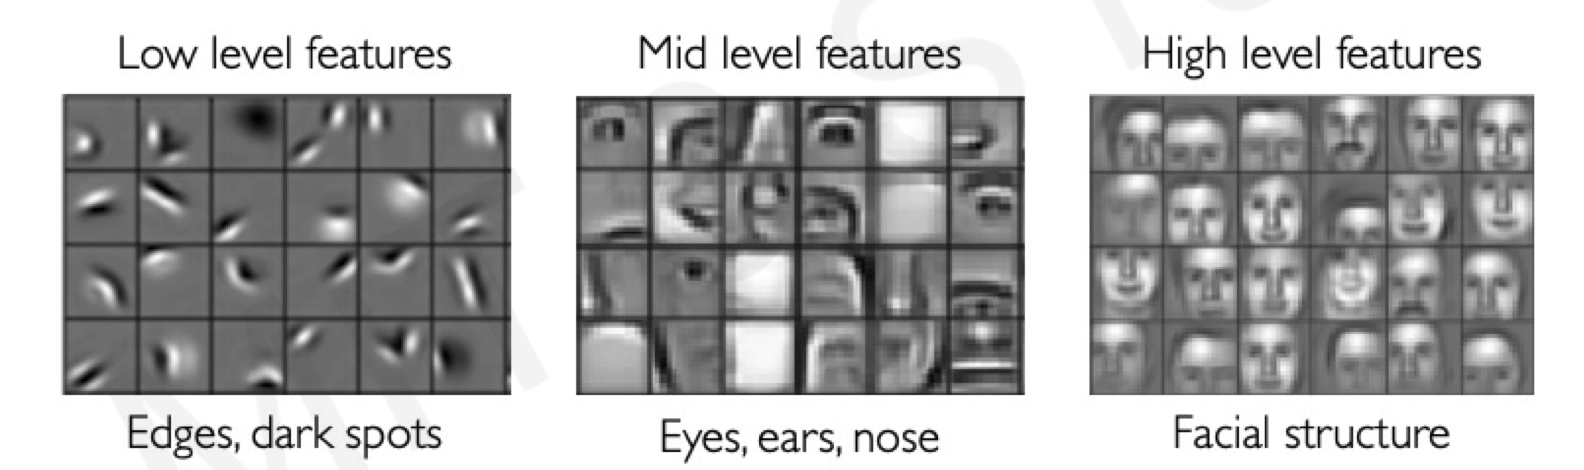
\includegraphics[width=0.85\textwidth]{images/Learning-Feature-Representation.png}
    \caption{Illustration of feature abstraction hierarchy in CNNs, from low-level (edges) to high-level (semantic object parts). Adapted from \cite{alexanderaminiMITIntroductionDeep2025}.}
    \label{fig:Hierarchy_of_Features}
\end{figure}
This hierarchy show why shallow layers are often more domain-specific, as they are prone to capturing texture or lighting, while deeper layer are more semantic and thus domain-invariant. Feature-space domain generalization methods like MixStyle \citep{zhouMixStyleNeuralNetworks2023} start their approach there.
Feature representations derived from CNNs, often form domain-specific clusters in the latent space. This in particular is problematic for Domain Generalization, where the models needs to learn representations that are invariant to such domain cues \citep{zhouDomainGeneralizationSurvey2022}.

\begin{figure}[!htb]
    \centering
    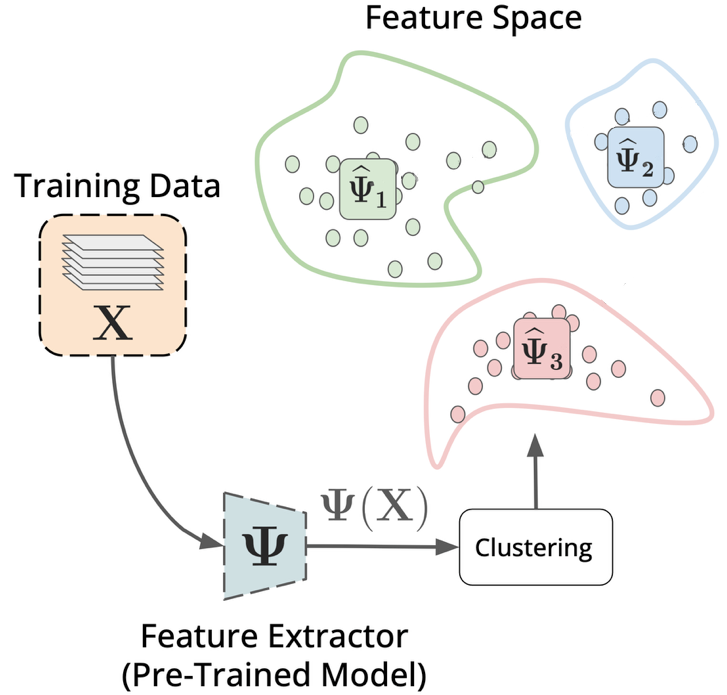
\includegraphics[height=0.33\textheight]{images/Pipeline-Feature_Space.png}
    \caption{A model pipeline showing input images from different domains processed by a pretrained feature extractor, producing clustered representations in feature space. Image from \cite{thomasWhatsLatentLeveraging2025}, modified.}
    \label{fig:Pipeline_Feature_Space}
\end{figure}
Clustered representations usually reflect the characteristics of the source domain. Without any intervention from the outside, models trained on these clustered representations might struggle to generalize to new domains.

One effective way to address this issue is by utilizing transfer learning, by reusing pretrained models.
\subsection{Transfer Learning}
Transfer learning refers to the process of leveraging knowledge obtained from one task or domain to improve performance on a different, yet related, task. In the context of computer vision, it often involves using models pretrained on large-scale datasets — such as ImageNet — and adapting them to new tasks with limited data.

This approach is particularly relevant to Domain Generalization, where the goal is to generalize to an unseen target domain without access to its data during training \citep{gulrajaniSearchLostDomain2020,liDeeperBroaderArtier2017}. Transfer learning can support this objective by providing models with general-purpose representations learned from diverse visual categories and conditions.

Convolutional Neural Networks (CNNs) pretrained on large datasets tend to capture a hierarchy of features as seen in figure \ref{fig:Hierarchy_of_Features} — from low-level structures like edges and textures to high-level semantic patterns. These pretrained networks are often used as feature extractors enabling downstream models to build upon robust and transferable representations rather than learning from scratch.
Furthermore, beyond improved sampling efficiency, transfer learning can also stabilize training and reduce overfitting, especially in cases where the available training data is limited or varies substantially across domains \citep{thomasWhatsLatentLeveraging2025}. Thus, transfer learning provides a useful foundation for addressing domain shift in Domain Generalization settings, even though it is not exclusive to them.

However, leveraging pretrained networks also requires careful handling — especially when it comes to controlling which parts of the network are updated during training. This leads to the concept of freezing, which helps maintain stable, domain-invariant representations.

\subsection{Freezing}
Freezing refers to the practice of preventing specific layers of a neural network from being updated during training. This is commonly applied in transfer learning to retain the general-purpose features learned by pretrained models, especially in the early convolutional layers.

In Domain Generalization, freezing can be used to improve the model's ability to generalize across domains. Specifically, it helps prevent the network from overfitting to the domain-specific features of the source domains — an issue particularly relevant when training on multiple diverse datasets. By keeping the early or mid-level layers fixed, the model is encouraged to rely on more generalizable representations rather than learning domain-specific features. A critical motivation for freezing in Domain Generalization arises from the use of Batch Normalization. Batch Normalization layers compute and update feature statistics (mean and variance) during training, which are sensitive to the distribution of the training data. In a multi-source setting, where training batches may contain samples from several domains, these statistics can become unstable or biased toward dominant domains. By freezing Batch Normalization layers, one can preserve the pretrained statistics and avoid learning domain-specific biases, thus supporting better generalization \citep{Goodfellow-et-al-2016,zhouMixStyleNeuralNetworks2023}.

Therefore, freezing is a strategic complement to transfer learning: while transfer learning brings in generalizable knowledge, freezing ensures that this knowledge is not overwritten during training on source domains. It has been used effectively in several recent Domain Generalization approaches such as MixStyle \citep{zhouMixStyleNeuralNetworks2023}.
\subsection*{Summary}
In summary, Domain Generalization provides a more demanding but often more practical solution than Domain Adaptation for creating models that are robust to the diverse and unpredictable domain shifts encountered in real-world scenarios.

Transfer Learning and Freezing can be used to supplement the training process, by providing a robust feature extraction backbone and by preventing the model from overfitting to the domain-specific features of the source domains.
